% tutorial.tex  -  a short descriptive example of a LaTeX document
%
% For additional information see  Tim Love's ``Text Processing using LaTeX''
% http://www-h.eng.cam.ac.uk/help/tpl/textprocessing/
%
% You may also post questions to the newsgroup <b> comp.text.tex </b> 

\documentclass[12pt]{article}			% For LaTeX 2e
						% other documentclass options:
						% draft, fleqn, openbib, 12pt

\usepackage{graphicx}	 			% insert PostScript figures
%% \usepackage{setspace}   % controllabel line spacing
%% If an increased spacing different from one-and-a-half or double spacing is
%% required then the spacing environment can be used.  The spacing environment 
%% takes one argument which is the baselinestretch to use,
%%         e.g., \begin{spacing}{2.5}  ...  \end{spacing}


% the following produces 1 inch margins all around with no header or footer
\topmargin	=10.mm		% beyond 25.mm
\oddsidemargin	=0.mm		% beyond 25.mm
\evensidemargin	=0.mm		% beyond 25.mm
\headheight	=0.mm
\headsep	=0.mm
\textheight	=220.mm
\textwidth	=165.mm
					% SOME USEFUL OPTIONS:
% \pagestyle{empty}			% no page numbers
 \parindent  15.mm			% indent paragraph by this much
 \parskip     2.mm			% space between paragraphs
% \mathindent 20.mm			% indent math equations by this much

\newcommand{\MyTabs}{ \hspace*{25.mm} \= \hspace*{25.mm} \= \hspace*{25.mm} \= \hspace*{25.mm} \= \hspace*{25.mm} \= \hspace*{25.mm} \kill }

\graphicspath{{../Figures/}{../data/:}}  % post-script figures here or in /.

					% Helps LaTeX put figures where YOU want
 \renewcommand{\topfraction}{0.9}	% 90% of page top can be a float
 \renewcommand{\bottomfraction}{0.9}	% 90% of page bottom can be a float
 \renewcommand{\textfraction}{0.1}	% only 10% of page must to be text

\linespread{1.2}
\alph{footnote}				% make title footnotes alpha-numeric

\title{Continuous Authentication}	% the document title
\author{{\bf Project report}{\bf}}
\date{}				% your own text, a date, or \today

% --------------------- end of the preamble ---------------------------

\begin{document}			% REQUIRED

\pagenumbering{roman}			% Roman numerals from abstract to text
\maketitle				% you need to define \title{..}
\thispagestyle{empty}			% no page number on THIS page 

\begin{center}

%A synopsis submitted in partial fulfillment of the requirements of the course \\[3ex]
{\Large CS812}\\[3ex]
{\Large}

{\large}
{\bf Under the guidance of }{\bf}\\[2ex]
Dr. K. G. Srinivasa\\
Professor\\
Department of Computer Science and Engineering\\
M. S. Ramaiah Institute of Technology\\[3ex]


{\bf Submitted by}{\bf}\\[2ex]
{\bf Soumya Gosukonda }{\bf} 1MS08CS119\\
{\bf Tribhuvanesh Orekondy }{\bf} 1MS08CS129\\[8ex]
{\large}


\includegraphics[scale=0.20]{msrit.png}\\
Department of Computer Science and Engineering\\
M. S. Ramaiah Institute of Technology\\
(Autonomous Institute Affiliated to VTU)\\
Bangalore - 560054
\end{center}

\newpage
\begin{abstract}			% beginning of the abstract

% TODO <-----ABSTRACT GOES HERE------>

Password based security is a commonly used measure to enforce valid authentication. Coupled with Iris and/or fingerprint based recognition, these systems, known as biometric authentication systems, strengthen this process of authentication. However, this is a one-time process and fails to provide continuous authentication. To illustrate the idea of Continuous Authentication (CA) consider a situation where the user has to leave her/his workstation unattended for a short period of time and forgets to lock it. In this time interval it is possible for an unauthorized user to gain access to the system and tamper with it. To avoid such a situation, continuous authentication can prove useful. 
This project aims to deliver a continuous authentication system based on face recognition and soft biometric traits, namely shirt colour. We plan to achieve this goal using the OpenCV library and a suitable mathematical model.


\end{abstract}				% end of the abstract
\newpage
\begin{center}
{\LARGE \bf Acknowledgements}
\\[6ex]
\end{center}
We would like to thank our project guide, Dr. K.G.Srinivasa, for his valuable and much-needed guidance and patience during the course of this project. We are grateful for the timely inputs we received from him, right from the start of the project.\\[2ex]
We are thankful to the Department of Computer Science and Engineering, and our Head of Department, Dr. R. Selvarani, for having provided us an opportunity to work on this project and enhance our skills in this field.\\[2ex]
We also thank the lab assistants and our friends for their immense help and suggestions that helped us further improve the project. 
\newpage				% start a new page
\tableofcontents			% create table of contents automatically
\newpage				% start a new page
\pagenumbering{arabic}			% Arabic page numbers from now on

\section{ Introduction }	% start the first numbered section

% <-------- INTRODUCTION -------->

\subsection{ General Introduction }
Static Authentication enables a user to log in to a session through his/her account by providing the required credentials at the beginning. This form of authentication doesn’t consider the possibility of tailgating when the authorized user is not present in front of the authenticated system. On the other hand, Continuous Authentication provides a solution by authenticating the user right from the initial stages of log-in through log-out. This is implemented by checking the facial features of the user during log in, followed by creating a template of the user containing his/her soft biometric traits, which in this case, is the colour of the user’s clothing [Niinuma et al]. 

\subsection{ Problem Definition }
Soft biometric traits don’t provide as high a level of confidence when compared to hard biometric traits. The problem here is to design a system by which the threshold of confidence in authenticating the user can be increased by intelligently verifying these hard biometric traits and then moving over to a soft biometrics verification by implementing a suitable mathematical model.


\section{Literature Survey }
%\subsection{ Continuous Authentication }

\subsection{ OpenCV }
OpenCV (Open Source Computer Vision Library) is a library of programming functions mainly aimed at real time computer vision, developed by Intel and now supported by Willow Garage. It is free for use under the open source BSD license. The library is cross-platform. It focuses mainly on real-time image processing. If the library finds Intel's Integrated Performance Primitives on the system, it will use these proprietary optimized routines to accelerate itself.

\subsection{ Face Detection }
OpenCV's face detector uses a method that Paul Viola and Michael Jones published in 2001 [1]. Usually called simply the Viola-Jones method, or even just Viola-Jones, this approach to detecting objects in images combines four key concepts:
\begin{itemize}
	\item{} Simple rectangular features, called Haar features
	\item{} An Integral Image for rapid feature detection
	\item{} The AdaBoost machine-learning method
	\item{} A cascaded classifier to combine many features efficiently
\end{itemize}

\subsubsection{ EigenFace }
Eigenface [2] consists of two phases: learning and recognition. In the learning phase, you give eigenface one or more face images for each person you want it to recognize. These images are called the training images. In the recognition phase, when you give eigenface a face image, it responds by telling you which training image is "closest" to the new face image.

Eigenface uses the training images to "learn" a face model. This face model is created by applying a method called Principal Components Analysis (PCA) to reduce the "dimensionality" of these images. Eigenface defines image dimensionality as the number of pixels in an image.

The lower dimensionality representation that eigenface finds during the learning phase is called a subspace. In the recognition phase, it reduces the dimensionality of the input image by "projecting" it onto the subspace it found during learning. "Projecting onto a subspace" means finding the closest point in that subspace. After the unknown face image has been projected, eigenface calculates the distance between it and each training image. Its output is a pointer to the closest training image. You can then look up which person that was to see whom eigenface has identified.

\subsection{ Soft Biometric Traits }
Soft Biometric Traits refers to features of the user that identify the user on a temporary basis [3]. These can refer to, but are not limited to, the following:
\begin{itemize}
	\item{} Physical: colour of skin, eyes and/or hair, presence of beard/moustache.
	\item{} Behavioural: gait, keystrokes.
	\item{} Adhered Human Characteristics: clothes colour, tattoos, accessories such as spectacles.
\end{itemize}

This approach has been well-researched and documented in \textit{Soft Biometric Traits for Continuous User Authentication} by Niinuma et al., Fujitsu Lab, 2010.

\section{Software Requirements Specification }
\subsection{ Introduction }

\subsubsection{ Purpose }
The purpose of this Software Requirements Specification is to provide a complete description of all the specifications and functions of the Continuous Authentication system as described above.

\subsubsection{ Scope of the Project }
Continuous authentication prevents the system from compromising the user's authenticity by continuously ensuring that the confidence in the identity of the user doesn't fall below a certain threshold. A video-feed from the web-cam is used to capture the user's traits throughout the session. A session here can be associated with the user logged-in to an e-mail or online banking account, or an account on the operating system itself.

\subsubsection{ Overview of Document }
The rest of this Software Requirements Specification proceeds with a general description of the project followed by the specific requirements of this software. 

\subsection{ General Description }
\subsubsection{ Project Perspective }
The Continuous Authentication system is designed as a stand-alone application which grants the user certain privileges at the time of successful log-in and continuously authenticates the user. The application enters into a lock-down mode in case an unauthorized  user attempts to use the authenticated user's privileges. 

\subsubsection{ Product Functions }
The Continuous Authentication system aims to provide the two primary functions:
\begin{itemize}
	\item To check the hard biometric traits of the user during the initial log-in stage and during certain periods after log-in till session ends.
	\item Continuously monitor the identity of the authenticated user and lock-down when required.
\end{itemize}

\subsubsection{ End users }
This application provides an added layer of security for users who wish to protect access to confidential information. Consequently, the user can rely on the system to ensure the privacy of his/her information.

\subsubsection{ General Constraints }
This application is constrained by the following:
\begin{itemize}
	\item The end-user's system should be capable of processing the real-time video-feed.
	\item The lighting conditions during usage to be similar to that captured by the training set.
	\item The system is incapable of performing a hard biometric recognition in case of occlusion.
\end{itemize}

\subsubsection{ Assumptions and Dependencies }
This application is assumes the following:
\begin{itemize}
	\item The user's system is equipped with a web-cam.
	\item The user is working in a sufficiently illuminated environment.
\end{itemize}

\subsection{ Specific Requirements }
\subsubsection{ Functional Requirements }
\begin{itemize}
	\item{\it Provide initial log-in, and verify user's password followed by the user's hard biometric traits. }
	\item{\it Create an account for a new user in the xml database and collect user's facial features and retrain the model. }
	\item{\it Create a user template with the user's soft biometric traits (shirt colour) once the user's face has been recognized with a minimum given confidence level.  }
	\item{\it Use the shirt-colour template to continuously verify the user's identity.  }
	\item{\it If the soft biometric verification falls below a certain threshold, restart face recognition of the user.  }
	\item{\it Lock-down in case of a tailgating unauthorized user. }
	%\item{\it A session time-out occurs in case the user logs in and then leaves the workstation unattended for a specified time limit. }
\end{itemize}

\subsubsection{ Software Requirements }
\begin{itemize}
\item C++ compiler (g++ 4.6.1)
\item OpenCV libraries
\item Drivers for web-cam
\item Python 2.7.1
\end{itemize}

\subsubsection{ Hardware Requirements }
\begin{itemize}
\item Web-cam with drivers supported by OpenCV, with a minimum resolution of 1.3MP
\item Memory : 2GB DDR2
\item Processor : A minimum of 3.0GhZ single core processor
\end{itemize}

\subsection{ Interface Requirements }
\subsubsection{ User Interface }
The user interface is provided with functions necessary to take as input the credentials of the user and display the live video-feed from the web-cam.

\section{ System Architecture and Design }  
\subsection{ Block diagram }
\begin{center}
    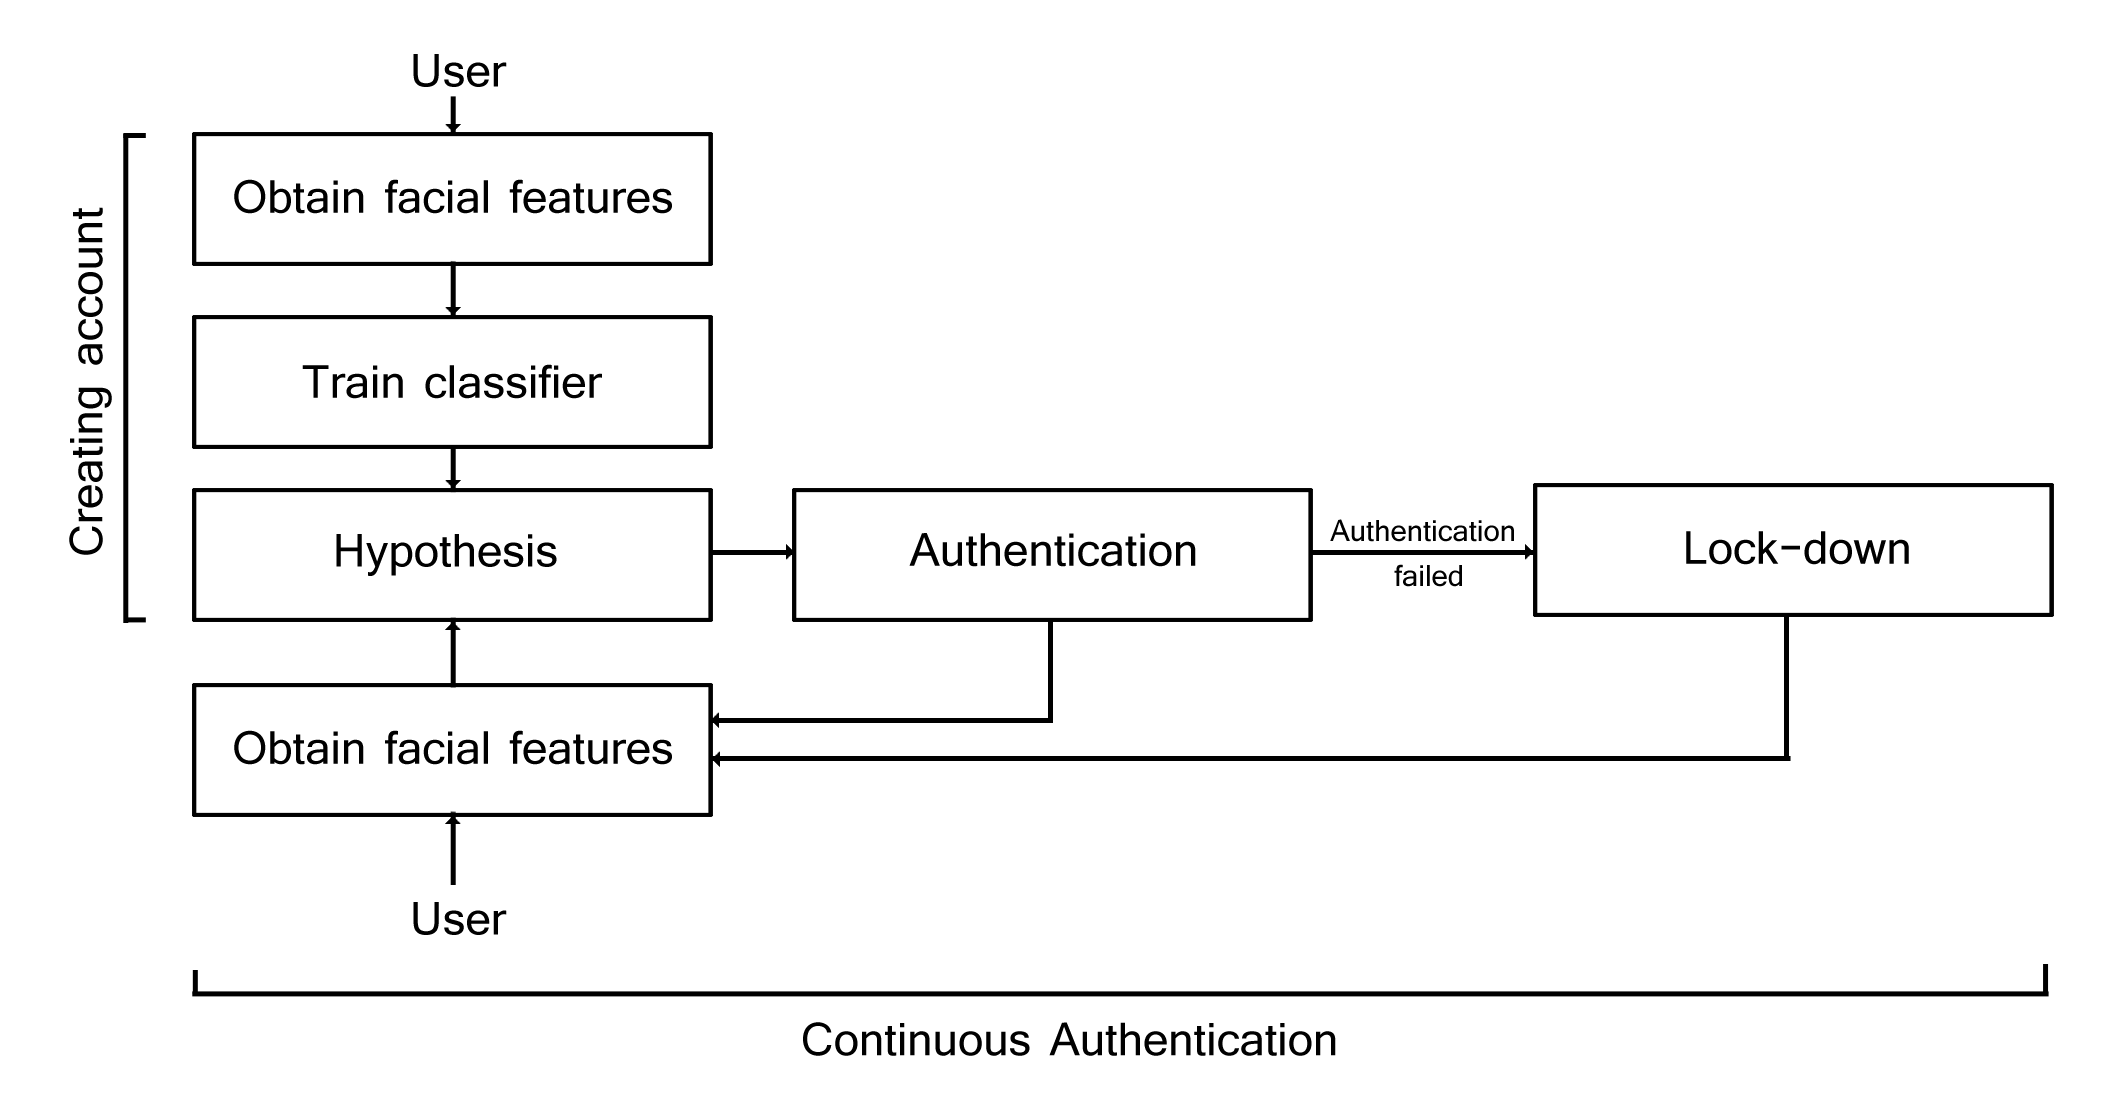
\includegraphics[scale=0.8]{block.png}
\end{center}

\section{ Detailed Design }
\subsection{ Data Persistence }
The persistent data in this system consists of:
\begin{itemize}
\item Training data set - Training data set consists of 51 equalized, grayscale images of each user stored in their respective directories. These are collected from a web-cam when a new user creates an account.% TO MENTION - resolution of pics
\item Eigenfaces data - This training data set is used to compute, using Principal Component Analysis, a set of "EigenFaces" representing the main differences between the training images. An "average face image" is computed and stored as \verb+avg_image.jpeg+. 
\item User-account data - User-account data refers to user-id, username, password stored in the form of a 160-bit hash string (SHA-1 encrypted).
\end{itemize}

An XML file names \verb+"face_data.xml"+ contains the integrated eigenfaces and user-account data. Its structure is as shown below:
\begin{verbatim}
-<opencv_storage>
	<nPersons> \textit{number of users} </nPersons>
	<personName_i> \textit{username of ith user} </personName_i>
	<nEigens>\textit{number of eigenfaces}</nEigens>
	<nTrainFaces>\textit{number of training images}</nTrainFaces>
	
	<trainPersonNumMat type_id="opencv-matrix">
		<rows>\textit{number of rows}</rows>
		<cols>\textit{number of columns}</cols>
		<dt>\textit{data type}</dt>
		<data>\textit{data}</data>
	</trainPersonNumMat>
	<eigenValMat type_id="opencv-matrix">
		<rows>\textit{number of rows}</rows>
		<cols>\textit{number of columns}</cols>
		<dt>\textit{data type}</dt>
		<data>\textit{data}</data>
	</eigenValMat>
	<projectedTrainFaceMat type_id="opencv-matrix">
		<rows>\textit{number of rows}</rows>
		<cols>\textit{number of columns}</cols>
		<dt>\textit{data type}</dt>
		<data>\textit{data}</data>
	</projectedTrainFaceMat>
\end{verbatim}

\subsection{ Module Description }
This section describes the various modules of the system which can be categorized as follows:
\begin{itemize}
\item Utilities
\item Face Detection
\item Soft Biometrics
\end{itemize}

\subsubsection { Utilities }
This module contains all the commonly used image processing functions that perform the following:

\begin{itemize}
\item Convert image to grayscale: Images captured by the webcam need to be converted to grayscale before being processed for computing Eigenfaces. It takes as input an IplImage pointer and returns pointer to the converted grayscale image. Its prototype is as follows:
\verb+IplImage* convertImageToGrayscale(IplImage* srcImage)+
\item Return image of the face in the frame defined by a CvRect datatype: Once a face is detected, the rectangular coordinates are saved into a CvRect datatype and the cropped image containing the face is returned to the IplImage pointer. Its prototype is as follows:
\verb+IplImage* cropImage(IplImage* srcImage, CvRect faceRect)+
\item Resize Image: The cropped image containing the face needs to be resized to a standard resolution. This function takes as input source image to be resized, a boolean datatype stating whether to preserve aspect ratio, and the new height and width to be resized to. Its prototype is as follows:
\begin{verbatim}
IplImage* resizeImage(IplImage* srcImage,
bool preserveAspectRatio = true, int newHeight = _faceHeight,
int newWidth = _faceWidth)
\end{verbatim}
\item Draw a box around the face: This funtion draws a box around the face as indicated by the coordinates it takes as input. This image is later displayed in a window. It also takes a colour value and pointer to the image on which to draw the box. Its prototype is as follows:
\verb+void drawBox(IplImage* image, CvRect rect, CvScalar colour)+
\end{itemize}

\subsubsection { Face Detection }
This module contains the function that detects a face given an image captured from the webcam. It uses the Viola-Jones Face detection algorithm by making a call to the OpenCV function - cvHaarDetectObjects(). It takes as input the image to detect a face in, and the Haar Classifier Cascade as defined in the respective XML file. This cascade file defines the features of the "object" to look for, in this case, the face. Its prototype is as follows:
\verb+CvRect detectFace(IplImage* image, CvHaarClassifierCascade* cascade)+

\subsubsection { Soft Biometrics }
This module contains all the functions related to Soft Biometric trait recognition, namely, shirt colour of the user.

\begin{itemize}
\item Obtain the colour type given the Hue (H), saturation(S), and Value(V) values of a pixel. Its prototype is as follows:
\verb+int getPixelColorType(int H, int S, int V);+

\item Create a shirt colour template for the session which contains information about the percentage of each (of 11 specified colour types) colour present in the region detected as shirt region. Its prototype is as follows:
\begin{verbatim}
map<string, float> createTemplate(CvCapture* capture,
CvHaarClassifierCascade* cascadeFace, int avgIterations)
\end{verbatim}
\item Obtain a session template for a user by detecting a face in the input image and further detecting the shirt region. If region is found the colour composition of the detected shirt frame is calculated and stored in the template. Its prototype is as follows:
\verb+map<string, float>  getTemplate( IplImage*, CvHaarClassifierCascade*, CvRect)+

\item Return the average of 5 shirt colour templates created for ascertaining the user's shirt colour. Its prototype is as follows:\\
\verb+map<string, float>  createAverage( vector< map<string, float> > )+

\item Calculate the corresponding sigmoid function value given afloating point input. Its prototype is as follows:
\verb+float sigmoid( float )+

\item Calculate the normalized root mean square value given the set of 5 templates and the average template as inputs. Its prototype is as follows: \\
\verb+float nrmsd( map<string, float>, map<string, float> )+

\item A function that manages the soft biometric traits recogition and is called from the main module. Its prototype is as follows:
\verb+int soft_main()+
\end{itemize}

%\subsection { Main Module }

\section{ Implementation }  
This project has been implemented in C/C++ along with the OpenCV library for the image processing and face detection and recognition algorithms. A minor script in Python (version 2.x) is also used to reorganize the training data and create a file which stores the pathnames of the image files in the training data set. The implementation of the Continuous Authentication System can be divided into three major modules as per the modes of operation: building the training data set, learning, and the continuous authentication mode.
\subsection { Building Training Data Set }
This mode is launched when a new user is creating an account at which point the system collects images of the user's face in an equalized, grayscale format and stores it with the file extension ".jpeg". For this, the system runs the Face detection module, and collects 51 face images, which are stored under the specified username along with the password encrypted into a hash string by the SHA-1 encryption algorithm. It moves into the learning mode as soon as the faces are collected. 
\subsection { Learning }
This mode is launched subsequently after the collection mode or can be specifically launched into by passing "--learn" as a command-line argument. In this mode, Eigenface uses the training images to "learn" a face model[6]. the training images of all users are loaded into the array \emph {nTrainFaces}, and Principal Component Analysis (PCA) is carried out to find a PCA subspace, which is a lower dimensionality representation[6]. Then the training images are projected onto the PCA subspace, by calling the built-in library function cvEigenDecomposite(). Following this, the resulting data, namely Eigenvalues, Eigenvectors, The average training face image, Projected faces and Person ID numbers, is stored into the XML file - "facedata.xml".    
\subsection { Continuous Authentication Mode }
This mode is the de-facto mode of operation. It involves requesting the user to login with his/her username and password. If the user's password matches the stored hash string from the XML file - "facedata.xml" the system proceeds to recognising the user's face from the webcam feed. If the entered password is wrong, then the program exits. If the user is recognized by the system, then he/she is granted access. Otherwise, the system enters a lockdown mode. After the confidence level reaches a peak of 99\% then it enters into the soft biometrics mode. In this mode, the system detects faces in the webcam feed and corresponding to the location of the face detects a shirt region below the face detected. The coordinates are stored in a CvRect type and a template is created for the session which will be used to further authenticate the user continuously. If the shirt detection level falls, then the system restarts the face recognition to verify if the user is still present.  

\section{ Testing }

\subsection{ Unit testing }
The two primary units that comprise the Continuous Authentication system were individually tested under real-world conditions.

\subsubsection{ Face Recognition }
\emph{ Requirement: } Faces should be accurately recognized\\
\emph{ Test: } A burst of 200 frames were collected with the user posing naturally with head movement\\
\emph{ Result: } An accuracy of 94\% was achieved.\\

\subsubsection{ Soft bio-metrics }
\emph{ Requirement: } The soft-biometrics captured should not vary by large from the initial captured template\\
\emph{ Test: } A burst of 200 frames was used with the user performing extreme movements\\
\emph{ Result: } An accuracy of 78\% was achieved\\

\subsection{ Performance testing } 
\emph{ Requirement: } The Continuous Authentication system should be able to meet real-time requirements on a system\\
\emph{ Test: } The code was tested on two systems - one with a Core 2 Duo processor at 3.0Ghz, and the other with a Core i5 processor at 2.66 Ghz\\
\emph{ Result: } The real time requirements was easily met on the Core i5 system, and the Core 2 Duo system, but with a minor lag\\

\subsection{ Security testing}
\emph{ Requirement: } One should not be able to log in without the right credentials, or be able to reverse engineer\\
\emph{ Test: } The passwords stored in the database should not be readable\\
\emph{ Result: } Since the SHA1 hashes of the users were stored in the database, it's harmless even if one tries to retrieve it\\

\subsection{ Compatibility testing }
\emph{ Requirement: } The CA system should be compatible with all the latest versions of the libraries used\\
\emph{ Test: } The code was compiled and executed on g++ 4.5-2.7, OpenCV versions 2.1-2.3 and 2 distributions of Linux\\
\emph{ Result: } The code successfully compiled and executed on all the above versions\\

\subsection{ Load Testing }
\emph{ Requirement: } The CA system should be able to lock-on on one sigle person and perform verification \\
\emph{ Test: } The system was tested with multiple people in the frame\\
\emph{ Result: } A lock-on was always performed on the largest-detected face in the frame\\

\subsection{ Integration testing}
\emph{ Requirement: } By integrating the two main components of Continuous Authentication, the system should successfully switch between them as and when needed\\
\emph{ Test: } A 10 minute run was conducted under real-world conditions\\
\emph{ Result: } The soft-biometrics mode was successfully able to switch to face recognition mode when confidence dropped below a certain threshold\\

\subsection{ System testing }
\emph{ Requirement: } A tail-gating unauthorized user should not be able to gain access for over 3-5 seconds\\
\emph{ Test: } A 10 minute run was conducted with the user and an imposter switching a number of times\\
\emph{ Result: } The imposter was able to gain access for over 5 seconds 2 times out of the 10 switches performed\\

\section{ Results }
The Continuous Authentication system was tested using 12 users in total, with 10 of those users having credentials registered in the database. Each user was logged in for a certain period in time, while the others tail-gated the authorized user. 

\begin{figure}
	\caption{Time taken - Face recognition vs. Soft biometrics}
	\centering
		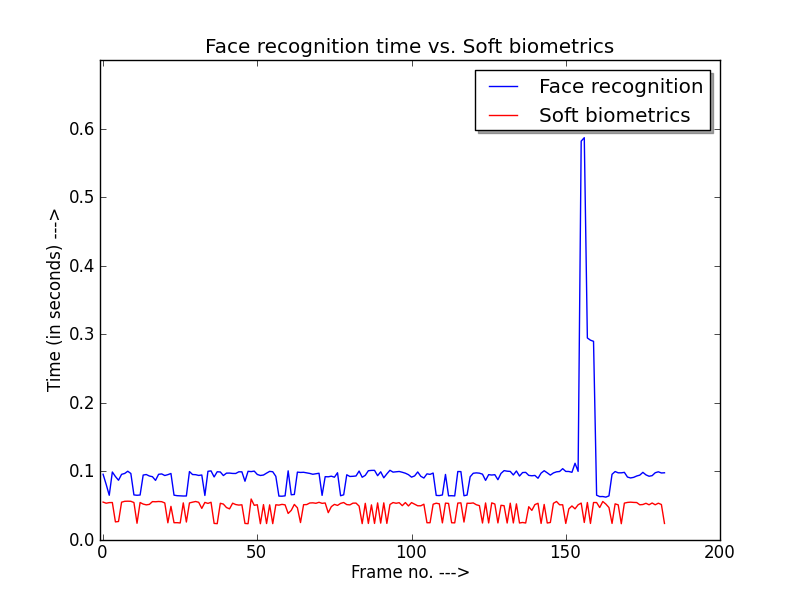
\includegraphics[scale=0.6]{img/face_vs_soft.png}
\end{figure}

\begin{figure}
	\caption{Face recognition accuracy - 94\%}
	\centering
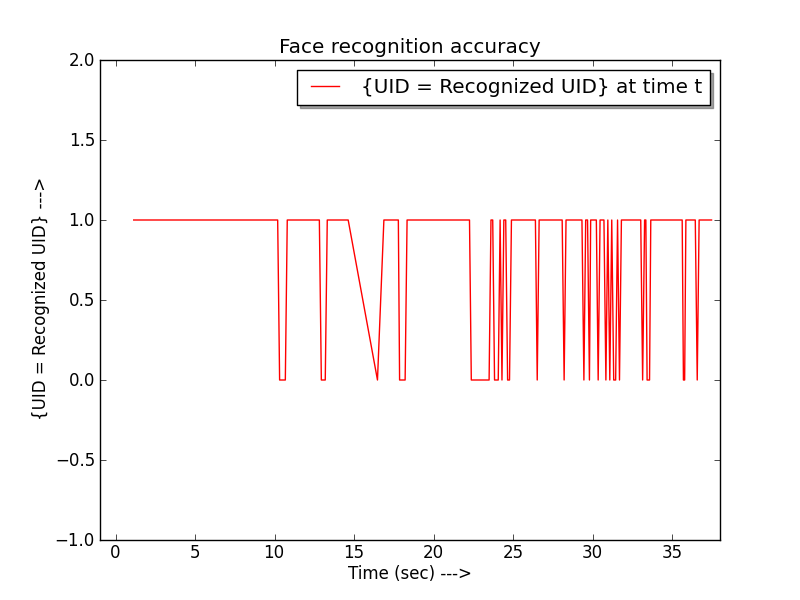
\includegraphics[scale=0.6]{img/face_rec_accuracy.png}
\end{figure}
\begin{figure}
	\caption{Mean vs. Recognized vs. Authorized}
	\centering
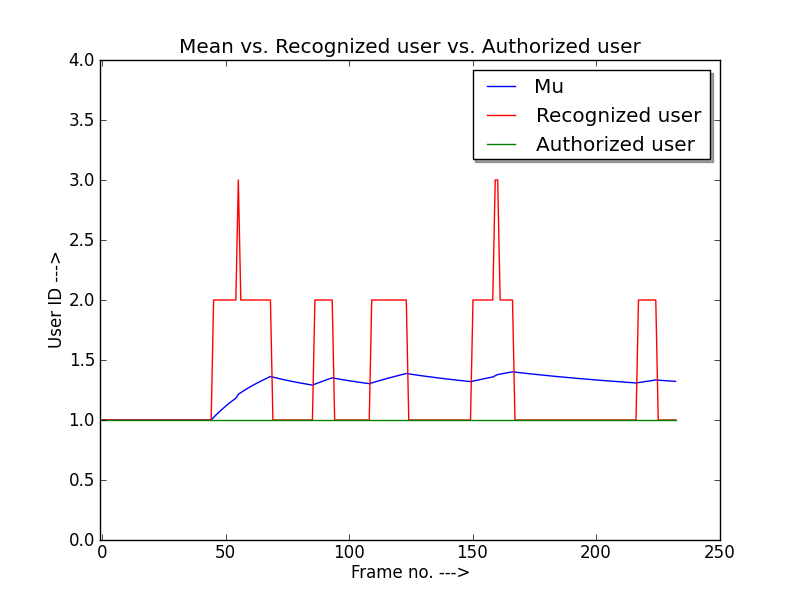
\includegraphics[scale=0.6]{img/mu_nearest_uid.png}
\end{figure}

\begin{figure}
	\caption{Initial uncertainity of user}
	\centering
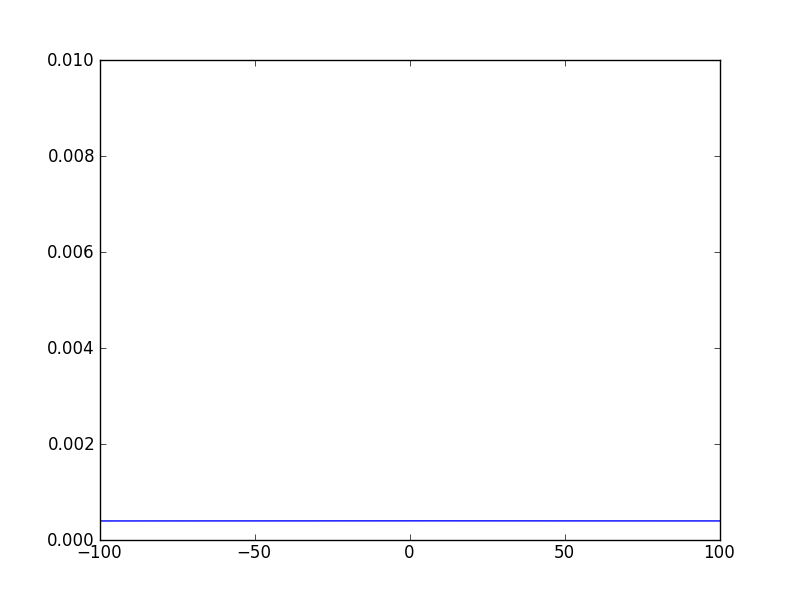
\includegraphics[scale=0.6]{img/mu_sig1.png}
\end{figure}

\begin{figure}
	\caption{Variance decreases in the subsequent frames if the authenticated user is present}
	\centering
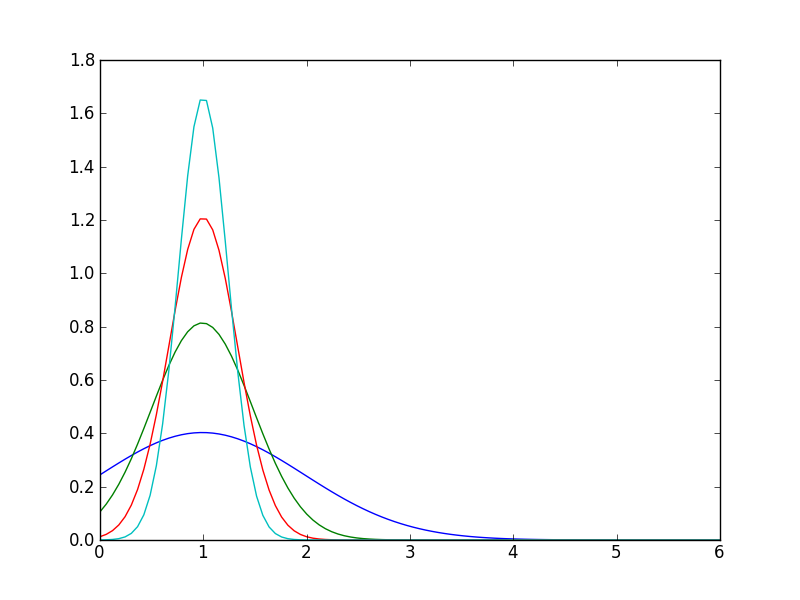
\includegraphics[scale=0.6]{img/mus_sig3.png}
\end{figure}
\begin{figure}
	\caption{Variance continues decreasing. Area under curve increases}
	\centering
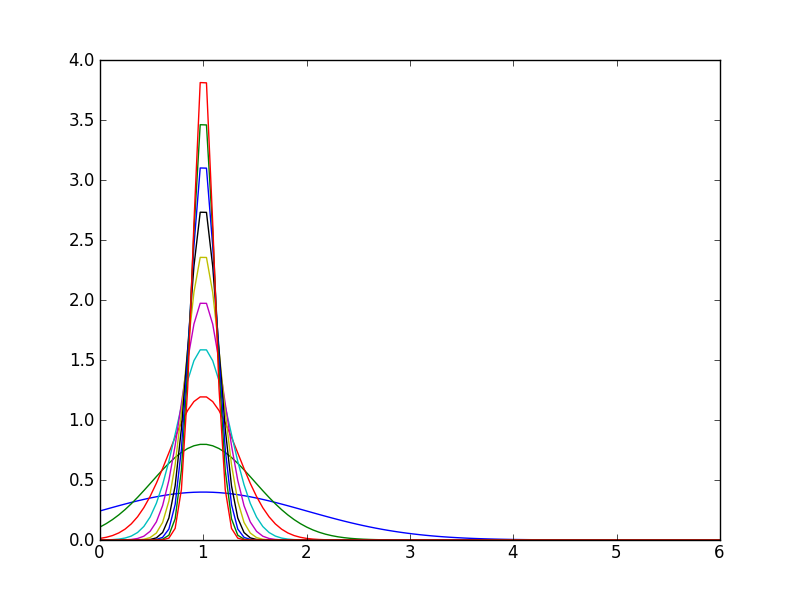
\includegraphics[scale=0.6]{img/mus_sig4.png}
\end{figure}

\begin{figure}
	\caption{Mean shifts as user changes}
	\centering
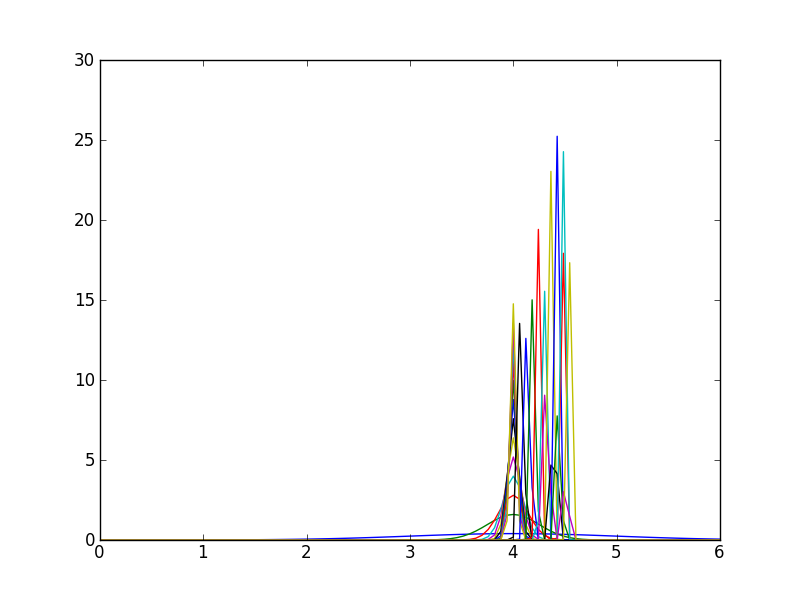
\includegraphics[scale=0.6]{img/mu_sig5.png}
\end{figure}

\begin{figure}
	\caption{Magnified version of previous figure}
	\centering
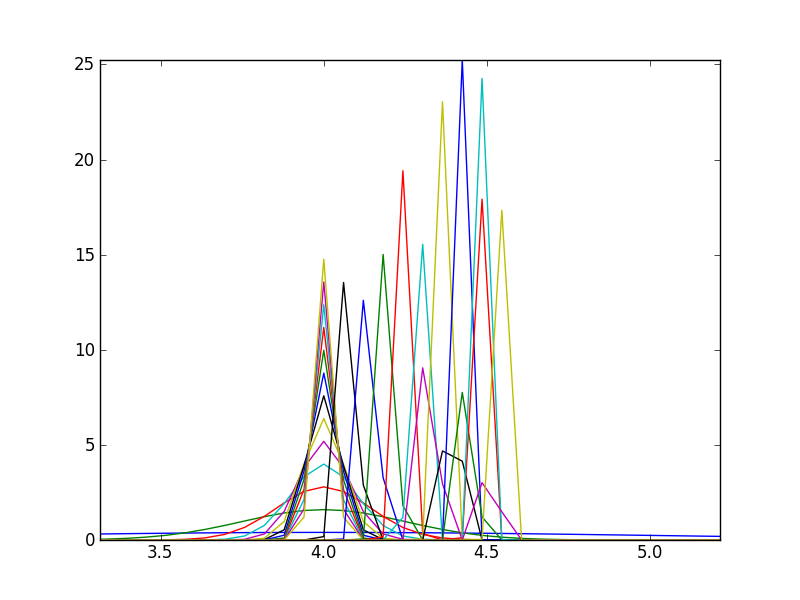
\includegraphics[scale=0.6]{img/mus_sig5.png}
\end{figure}

\newpage
\section{ Conclusion and Future Enhancements }
\subsection {Conclusion}
Need for biometric authentication arose from the fact that other security measures such as password and/or a smart ID card are prone to theft or loss. Biometrics depend on utilising features a user already possesses, that can uniquely identify a user atleast for a given session. However, using biometric identification has its downfalls. Since the characteristic of biometric traits is that they are not secretive, unlike a password, they can be gathered anywhere by an imposter and reconstructed for the authentication system to gain access. For example, a fingerprint left behind on some surface, can be picked up by imposters and reconstructed in front of the sensors. Even for face recognition systems, it is possible to fool the system by showing a photograph of the user or manipulating the video feed of the system. Countermeasures exist for such instances, such as, 3d reconstruction of face from more than two cameras or ensuring that the video feed cannot be manipulated. However, these measures make it a costly solution. Therefore, it can be concluded that biometric mode of authentication should be used more as a support system along with password/ smartID systems, to strengthen the authentication process, rather than a standalone mode of authentication.   

\subsection {Future Enhancements}
The following can be implemented in the future to enhance this system:
\begin{itemize}
\item Support for multiple users sharing a certain account; this may require a "biometric handoff" to occur between users.
\item Improve accuracy of face recognition under varied lighting conditions by implementing recognition using a different approach such as fuzzy logic.
\item Make provision for recognizing any kind of tampering occuring to the video feed, so as to prevent authenticating imposters. This can be done by restricting access to the webcam feed via parameters that define access to it.
\end{itemize}


\section{ References }
[1] Paul Viola, Michael Jones. Robust Real-time Object Detection. \textit {Second International Workshop on Statistical and Computational Theories of Vision - Modeling, Learning, Computing, and Sampling} (Vancouver, Canada), July 13, 2001. 

[2] Matthew Turk, Alex Pentland. Eigenfaces for Recognition. \textit {Journal of Cognitive Neuroscience} (Massachusetts Institute of Technology), 1991. 

[3] A.K. Jain, S.C. Dass, K. Nandakumar. Soft Biometric Traits for Personal Recognition Systems. \textit{ International Conference on Biometric Authentication.} 2004.
 
[4] Niinuma et al. Soft Biometric Traits for Continuous User Authentication. \textit{Fujitsu Lab}. 2010.

[5] Andrew J. Klosterman, Gregory R. Ganger. Secure Continuous Biometric-Enhanced Authentication. May 2000.

[6] Seeing With OpenCV, Part 5: Implementing Eigenface. by Robin Hewitt : \verb+http://www.cognotics.com/opencv/servo_2007_series/part_5/index.html+ \textit { Article from SERVO Magazine, May 2007. } 

\section{ Appendix }
\subsection{ Screen Snapshots}

% \section{ Applications }  
\end{document}				% REQUIRED

